\begin{figure}
    \centering
    \begin{small}
    \begin{sc}
    \begin{tikzpicture}[node distance=0cm, auto]
    \tikzstyle{header} = [text centered]
    \tikzstyle{pict} = [inner sep=4px]
    \tikzstyle{arrow} = [thick,->,-{Latex[scale=1]}]
    
    \node [header, right] (selection) {\makecell[c]{Sampling\\selection}};
    \node [header, right=1.4cm of selection] (patches) {\makecell[c]{Extracted\\patches}};

    \node [pict, below=of selection, label={[align=right]left:Grid\\sampling}] (ssel) {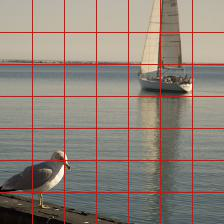
\includegraphics[width=1.8cm]{figures/teaser/1.jpg}};
    \node [pict, below=of ssel, label={[align=right]left:Elastic\\sampling}] (esel) {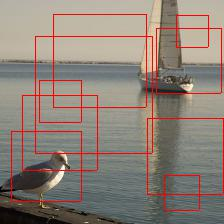
\includegraphics[width=1.8cm]{figures/teaser/3.jpg}};

    \node [pict] at (ssel -| patches) (sx) {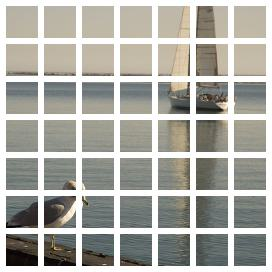
\includegraphics[width=1.8cm]{figures/teaser/2.jpg}};
    \node [pict] at (esel -| patches) (ex) {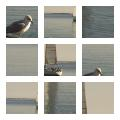
\includegraphics[width=1.8cm]{figures/teaser/4.jpg}};

    \draw [arrow] (ssel) -- (sx);
    \draw [arrow] (esel) -- (ex);
    \end{tikzpicture}
    \end{sc}
    \end{small}
    \afterplot
    \caption{\textbf{Grid vs. elastic sampling:} patch sampling with arbitrary patch positions and scales creates new possibilities for more effective and efficient vision transformers.}
    \label{fig:teaser}
    \vspace{-0.1in}
\end{figure}